%%%%%%%%%%%%%%%%%%%%%%%%%%%%%%%%%%%%%%%%%%%%%%%%%%%%%%%%%%%%%%%%%%%%%%
% Lớp 11 | Đường thẳng, mặt phẳng. Quan hệ song song trong | Hình lăng trụ và hình hộp (xiên)
% Dạng 1H4?5-2: Bài toán về hình lăng trụ (xiên)
% Số câu: 29  (sinh tự động bởi tach_cau.py; từ nay thầy sửa trực tiếp file này)
%%%%%%%%%%%%%%%%%%%%%%%%%%%%%%%%%%%%%%%%%%%%%%%%%%%%%%%%%%%%%%%%%%%%%%

%%%%%%%%%%%%%%%% TRẮC NGHIỆM 4 PHƯƠNG ÁN %%%%%%%%%%%%%%%%

% nguồn: Ok_TracNghiemLop11_Lan1
\begin{ex}%[1H4N5-2]%[ma:1812642c]
	Cho hình lăng trụ $ABC.A'B'C'$. Trong các khẳng  định sau, khẳng định nào là khẳng định $\textbf{sai}$?
	\choice 
		{$\left(ABC\right)  \parallel \left(A_1B_1C_1\right)$}
		{$AA_1  \parallel \left(BCC_1\right)$}
		{$AB \parallel  \left(A_1B_1C_1\right)$}
		{\True $AA_1B_1B$  là hình chữ nhật}
	\loigiai{ 
		Vì mặt bên $AA_1B_1B$ là hình  bình hành, còn nó là hình chữ nhật nếu $ABC.A'B'C'$ là hình lăng trụ đứng.
	} 
\end{ex}

% nguồn: Ok_TracNghiemLop11_Lan1
\begin{ex}%[1H4N5-2]%[ma:b6922ae0]
	Cho hình lăng trụ $ABCD.A'B'C'D'$. Mệnh đề nào  dưới đây là \textbf{sai}?
	\choice 
		{mp$\left( AA'B'B \right)$ song song với  mp$\left( CC'D'D \right)$}
		{\True Diện tích các mặt bên đều  bằng nhau}
		{Các cạnh  bên $AA'$ và $CC'$ song song nhau}
		{Hai mặt phẳng đáy có diện tích bằng  nhau}
	 \loigiai{\immini
		{ 
		Vì các mặt bên của hình lăng trụ $ABCD.A'B'C'D'$ là hình  bình hành, và ba kích thước chiều dài, chiều rộng, chiều cao của hình lăng trụ $ABCD.A'B'C'D'$ có thể khác khau nên diện tích các mặt bên có thể không bằng nhau.
		 }
		 {
		\begin{tikzpicture}[line join=round,line cap=round,scale=0.8]
				 \path
					(0,0) coordinate  (A)
					(3,0)  coordinate (B)
					 (4,2) coordinate (C)
					 (1,2) coordinate (D)
					 (0.5,3) coordinate (A')
					(3.5,3) coordinate (B') 
					(4.5,5) coordinate (C') 
					(1.5,5)  coordinate (D');
				\draw (A)--(B)--(C) 
					(A')--(B')--(C')--(D')--cycle (A)--(A') 
					 (B)--(B')
					(C)--(C'); 
				\draw[dashed] (A)--(D)--(C) 
					 (D)--(D');
				\foreach \i/\g in {A/-135,B/-45,C/0,D/180,A'/180,B'/0,C'/0,D'/135}{\draw[fill](\i)  circle (1pt)
					($(\i)+(\g:3mm)$)  node[scale=1]{$\i$};}
			\end{tikzpicture}
		} 
	} 
\end{ex}

% nguồn: Ok_TracNghiemLop11_Lan1
\begin{ex}%[1H4N5-2]%[ma:a5f2b68a]
	\immini{Cho hình lăng trụ $ABC.A'B'C'$. Gọi $M$, $N$, $P$ theo thứ tự là trung điểm của các cạnh $AA'$, $BB'$, $CC'$ (hình vẽ  bên).
	Mặt phẳng $\left(MNP\right)$ song song  với mặt phẳng nào sau đây?
	\choice 
		 {$\left(A'C'C\right)$}
		 {$\left(BMN\right)$}
		 {$\left(BCA'\right)$}
		 {\True $\left(ABC\right)$}
		}{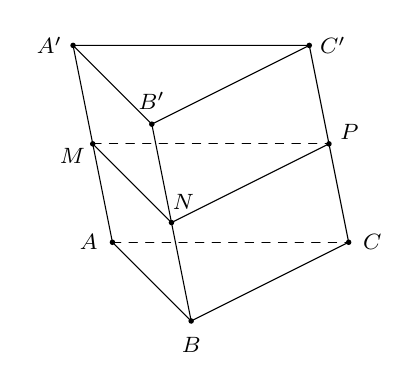
\begin{tikzpicture}[scale=1,font=\footnotesize,line join=round,line cap=round,>=stealth]
		\path (0,0) coordinate (A) 
			(3,0)  coordinate (C)
			(1,-1)  coordinate (B)
			(-0.5,2.5) coordinate (h); 
		\foreach \p  in {A,B,C}{\draw (\p)--(\p)--+(h) coordinate (\p');}
		\path (barycentric cs:A=1,A'=1) coordinate (M) 
			(barycentric cs:B=1,B'=1) coordinate (N) 
			(barycentric  cs:C=1,C'=1) coordinate (P);
		\draw (A')--(B')--(C')--cycle  (A)--(B)--(C)
			 (M)--(N)--(P);
		\draw[dashed] (A)--(C) 
			 (M)--(P);
		\foreach \p/\g in {A/180,B/-90,C/0,A'/180,B'/90,C'/0,M/210,N/60,P/30} \fill[black] (\p)  circle (1pt)+(\g:0.3) node{$\p$};
	\end{tikzpicture}
		} 
	 \loigiai{
	 Ta có $\heva{&MN\parallel AB \\&NP\parallel BC \\&MN\cap NP=N \\&AB\cap BC=B}\Rightarrow \left(MNP\right)\parallel \left(ABC\right)$.}
\end{ex}

% nguồn: Ok_TracNghiemLop11_Lan1
\begin{ex}%[1H4N5-2]%[ma:403657c7]
	Cho hình lăng trụ $ABC.A'B'C'$. Gọi $F$, $I$ và $N$ lần lượt  là trung điểm của các cạnh $AA'$, $BB'$ và $CC'$. Tìm khẳng định đúng.
	 \choice
		{  \True $(FIN)\parallel(A'B'C')$}
		{ $(FIN)\parallel(A'BC)$} 
		{ $(FIN)\parallel(BCC'B')$} 
		{  $(FIN)\parallel(AB'C')$}
	 \loigiai{
		\begin{center}
			\begin{tikzpicture}[scale=1,>=stealth,font=\footnotesize,line join=round,line cap=round]
					\path (0,0) coordinate (A') 
						 (4,0) coordinate (C')
						(-50:2.5) coordinate (B') 
						($(A')+(60:5)$) coordinate  (A)
						 ($(B')+(60:5)$) coordinate (B)
						($(C')+(60:5)$) coordinate  (C)
						 ($(B)!0.5!(B')$) coordinate (I)
						($(C)!0.5!(C')$) coordinate  (N)
						($(A')!1/2!(A)$)  coordinate (F);
					\draw (A')--(B')--(C')--(C)--(A)--cycle  (A)--(B)--(C)
						(B)--(B') 
						(F)--(I)--(N); 
					\draw[dashed] (C')--(A') 
						 (F)--(N);
					 \foreach \x/\g in {A'/180,B'/-90,C'/0,B/70,A/180,C/0,F/180,I/180,N/0
						}  \fill[black](\x) circle (1pt)+(\g:.3) node{$\x$};
				\end{tikzpicture}
		\end{center}
		Vì $F$, $I$ và $N$ lần lượt là  trung điểm của các cạnh $AA'$, $BB'$ và $CC'$ nên suy ra $$\heva{&FI\parallel A'B'\\&IN\parallel B'C'}\Rightarrow\heva{&FI\parallel (A'B'C')\\&IN\parallel(A'B'C').}$$
		Mà $FI\cap  IN=I$ nên $(FIN)\parallel(A'B'C')$.
	 }
\end{ex}

% nguồn: Ok_TracNghiemLop11_Lan1
\begin{ex}%[1H4N5-2]%[ma:b369c939]
	\immini[thm]{Cho  hình lăng trụ tam giác $ABC.A'B'C'$ như hình vẽ.
	Xác định hình chiếu của điểm $A$ trên mặt  phẳng $(A'B'C')$ theo phương $CC'$.
	 \choice
		 {$M'$}
		{\True  $A'$}
		 {$C'$}
		{$A$}} 
		{\begin{tikzpicture}[scale=0.8,font=\footnotesize,line join=round,line cap=round,>=stealth]
		\path 
			(0,0) coordinate  (A')
			 ($(A')+(-45:3)$) coordinate (B')
			 ($(A')+(0:4)$) coordinate (C')
			(80:3)  coordinate (z)
			 ($(A')+(z)$) coordinate (A)
			($(B')+(z)$) coordinate  (B)
			 ($(C')+(z)$) coordinate (C);
		 \draw
			 (B)--(A)--(C)
			(A')--(B')--(C')--(C)--(B)--(A)--(A') 
			(B)--(B'); 
		\draw[dashed] 
			(C')--(A'); 
		\foreach \x/\g in  {A/180,B/-135,C/0,A'/180,B'/-135,C'/0}
		\fill[black] (\x) circle  (0.6pt)+(\g:.4) node{$\x$};
	\end{tikzpicture}
		 }
	 \loigiai{
		Vì $ABC.A'B'C'$ là hình lăng trụ nên  $AA'\parallel BB'\parallel CC'$.\\
		Vì $A'$ thuộc mặt phẳng $(A'B'C')$ nên $A'$ là hình chiếu của $A$ trên mặt phẳng $(A'B'C')$  theo phương $CC'$.
	 }
\end{ex}

% nguồn: Ok_TracNghiemLop11_Lan1
\begin{ex}%[1H4H5-2]%[ma:05888efe]
	Cho hình lăng trụ $ABC.A'B'C'$. Gọi $I$, $J$, $K$ lần lượt là trọng tâm của các tam giác $ABC$, $ACC'$, $A'B'C'$.  Mặt phẳng nào sau đây song song với mặt phẳng $\left(IJK\right)$?
	 \choice
		{$\left(AA'C\right)$} 
		{$\left(A'BC'\right)$} 
		 {$\left(ABC\right)$}
		{\True  $\left(BB'C'\right)$}
	\loigiai{ 
	\immini{Gọi $M$, $N$, $E$ lần  lượt là trung điểm của $BC$, $CC'$, $B'C'$.\\
		Khi  đó, $\dfrac{AI}{IM}=\dfrac{AJ}{JN}=2\Rightarrow IJ\parallel MN$.\hfill $(1)$\\
		 Trong $\left(AA'ME\right)$ ta có $\dfrac{AI}{IM}=\dfrac{A'K}{KE}=2\Rightarrow IK\parallel ME$.\hfill $(2)$\\
		Ta  có $MN, ME\subset (BB'C'C)\equiv (BB'C')$.\hfill $(3)$\\
		Từ $(1)$, $(2)$ và $(3)$ suy ra $(IJK)\parallel (BB'C')$.}{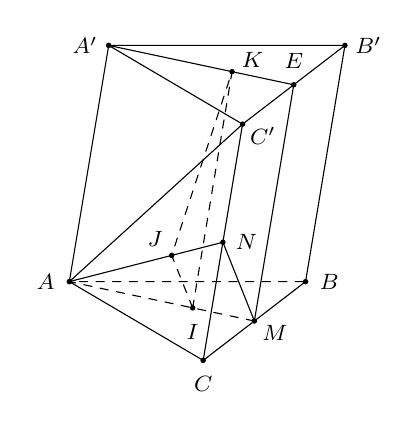
\begin{tikzpicture}[scale=1,font=\footnotesize,line join=round,line cap=round,>=stealth]
		\path (0,0) coordinate (A) 
			 (3,0) coordinate (B)
			 (1.7,-1) coordinate (C)
			(0.5,3)  coordinate (h);
		\foreach \p in {A,B,C}{\draw (\p)--(\p)--+(h) coordinate  (\p');}
		 \draw (A')--(B')--(C')--cycle (A)--(C)--(B);
		 \path (barycentric cs:A=1,B=1,C=1) coordinate (I)
			 (barycentric cs:A=1,C=1,C'=1) coordinate (J)
			(barycentric cs:A'=1,B'=1,C'=1)  coordinate (K)
			(barycentric cs:B=1,C=1)  coordinate (M)
			(barycentric cs:C'=1,C=1) coordinate (N) 
			(barycentric  cs:B'=1,C'=1) coordinate (E);
		 \draw[dashed] (M)--(A)--(B)
			 (I)--(J)--(K)--cycle;
		\draw  (A')--(E)--(M)--(N)--(A)--(C');
		\foreach  \p/\g in {A/180,C/-90,B/0,A'/180,C'/-30,B'/0,I/-90,J/135,K/30,M/-30,N/0,E/90} \fill[black] (\p) circle (1pt)+(\g:0.3) node{$\p$};
	\end{tikzpicture}
		} 
	 }
\end{ex}

% nguồn: Ok_TracNghiemLop11_Lan1
\begin{ex}%[1H4H5-2]%[ma:fe4d2dc3]
	Cho hình lăng trụ $ABC.A'B'C'$  (như hình vẽ)
	\begin{center}
		\begin{tikzpicture}[scale=1,font=\footnotesize,line join=round,line cap=round,>=stealth]
				\def\ac{4} 
				 \def\ab{2}
				 \def\ben{5}
				\def\gocnghieng{75} 
				\def\gocA{50} 
				\coordinate[label=left:$A$] (A) at (0,0); 
				\coordinate[label=right:$C$] (C) at  (\ac,0);
				 \coordinate[label=below left:$B$] (B) at (-\gocA:\ab);
				 \coordinate[label=left:$A'$] (A') at ($(A)+(\gocnghieng:\ben)$);
				\coordinate[label=below left:$B'$]  (B') at ($(B)-(A)+(A')$);
				\coordinate[label=right:$C'$] (C') at ($(C)-(A)+(A')$); 
				\coordinate[label=left:$D$] (D)  at ($(A)!0.5!(A')$);
				\coordinate[label=below left:$E$] (E)  at ($(B)!0.5!(B')$);
				\coordinate[label=above right:$F$]  (F) at ($(C)!0.5!(C')$);
				\coordinate  (M) at ($(C)!0.5!(B)$);
				\coordinate[label=below:$G$] (G)  at ($(A)!2/3!(M)$);
				 \draw (A')--(A)--(B)--(C)--(C')--(A')--(B')--(C')
					(B)--(B') 
					(D)--(E)--(F); 
				\draw[dashed]  (A)--(C)
					 (D)--(F)
					(A)--(M); 
				\foreach \diem in  {A,B,C,A',B',C',D,E,F,M,G} \fill (\diem) circle (1pt);
			\end{tikzpicture}
	\end{center}
	Lấy các điểm $D$, $E$, $F$ lần lượt là trung điểm của $AA'$, $BB'$, $CC'$ và điểm $G$ là trọng tâm  của tam giác $ABC$. Mệnh đề nào sau đây đúng?
	 \choice
		{$(DEB)\parallel  (A'B'F)$}
		{$(EFG)\parallel (BCD)$} 
		{\True $(DB'C')\parallel (AEF)$} 
		{$(DEG)\parallel (A'B'C)$} 
	 \loigiai{
		\begin{center}
			\begin{tikzpicture}[scale=1,font=\footnotesize,line join=round,line cap=round,>=stealth]
					\def\ac{4} 
					\def\ab{2} 
					\def\ben{5} 
					 \def\gocnghieng{75}
					 \def\gocA{50}
					 \coordinate[label=left:$A'$] (A) at (0,0);
					 \coordinate[label=right:$C'$] (C) at (\ac,0);
					 \coordinate[label=below left:$B'$] (B) at (-\gocA:\ab);
					 \coordinate[label=left:$A$] (A') at ($(A)+(\gocnghieng:\ben)$);
					\coordinate[label=below  left:$B$] (B') at ($(B)-(A)+(A')$);
					\coordinate[label=right:$C$] (C') at ($(C)-(A)+(A')$); 
					\coordinate[label=left:$D$] (D) at  ($(A)!0.5!(A')$);
					\coordinate[label=below left:$E$]  (E) at ($(B)!0.5!(B')$);
					\coordinate[label=above right:$F$]  (F) at ($(C)!0.5!(C')$);
					\coordinate  (M) at ($(C)!0.5!(B)$);
					\coordinate[label=below:$G$] (G) at  ($(A)!2/3!(M)$);
					\draw (A')--(A)--(B)--(C)--(C')--(A')--(B')--(C') 
						 (B)--(B')
						 (D)--(E)--(F)
						 (A')--(E)
						(D)--(B); 
					\draw[dashed]  (A)--(C)
						(D)--(F) 
						 (F)-- (A')
						 (A)--(M)
						 (D)--(C);
					 \foreach \diem in {A,B,C,A',B',C',D,E,F,M,G} \fill (\diem) circle (1pt);
				\end{tikzpicture}
		\end{center}
	Ta có các tứ giác $B'C'FE$; $B'DAE$ là hình bình hành  nên $B'C'\parallel (AEF)$ và\\ $B'D\parallel (AEF)$$\Rightarrow (DB'C')\parallel (AEF)$.}
\end{ex}

% nguồn: Ok_TracNghiemLop11_Lan1
\begin{ex}%[1H4H5-2]%[ma:3e67f644]
	 \immini{
	Cho  hình hộp $ABCD.A'B'C'D'$. Khẳng định nào sau đây \textbf{sai}?
	\choice 
		{$AB'C'D$ và $A'BCD'$ là hai hình bình hành  có chung một đường trung bình}
		 {$BD'$ và $B'C'$ chéo nhau}
		 {$A'C$ và $DD'$ chéo nhau}
		{\True $DC'$ và $AB'$ chéo nhau} 
		 }{
		\begin{tikzpicture}[scale=.6,font=\footnotesize,line join=round,line cap=round,>=stealth]
				 \path
					(0,0) coordinate (A) 
					(4,0) coordinate  (B)
					(-1.5,-1.5) coordinate  (D)
					($(B)+(D)-(A)$) coordinate  (C)
					 ($(A)!0.5!(C)$) coordinate (O)
					($(O)+(0,5)$) coordinate (A') 
					($(A')+(B)-(A)$) coordinate  (B')
					($(A')+(C)-(A)$) coordinate  (C')
					($(A')+(D)-(A)$) coordinate  (D');
				\draw (B)--(C)--(D) 
					(A')--(B')--(C')--(D')--(A') 
					 (B)--(B')
					 (C)--(C')
					(D)--(D'); 
				 \draw[dashed](B)--(A)--(D)
					(A')--(A); 
				\foreach  \x/\g in{A/150,B/0,C/-90,D/-90,A'/90,B'/0,C'/0,D'/180}
				 \fill[black](\x) circle (1pt)
					($(\x)+(\g:6mm)$) node{$\x$}; 
			\end{tikzpicture}
		 }
	 \loigiai{
		$DC'$ và $AB'$  song song với nhau.
	 }
\end{ex}

% nguồn: Ok_TracNghiemLop11_Lan1
\begin{ex}%[1H4V5-2]%[ma:57f4ffc1]
	Cho hình lăng trụ $ABC.A'B'C'$. Gọi $I$, $J$, $K$ lần lượt là trọng tâm của các tam giác  $ABC$, $ACC'$, $A'B'C'$. Mặt phẳng nào sau đây song song với mặt phẳng $(IJK)$?
	\choice 
		 {$(AA'C)$}
		 {$(A'BC')$}
		 {$(ABC)$}
		{\True $(BB'C')$} 
	\loigiai{ 
		\begin{center}
			\begin{tikzpicture}[scale=1,font=\footnotesize,line join=round,line cap=round,>=stealth]
					\def\ac{4} 
					 \def\ab{2}
					 \def\ben{4}
					\def\gocnghieng{75} 
					 \def\gocA{50}
					\coordinate[label=left:$A$]  (A) at (0,0);
					\coordinate[label=right:$C$] (C)  at (\ac,0);
					\coordinate[label=below  left:$B$] (B) at (-\gocA:\ab);
					\coordinate[label=left:$A'$] (A')  at ($(A)+(\gocnghieng:\ben)$);
					\coordinate[label=below left:$B'$]  (B') at ($(B)-(A)+(A')$);
					\coordinate[label=right:$C'$]  (C') at ($(C)-(A)+(A')$);
					\coordinate[label=below  right:$M$] (M) at ($(C)!0.5!(B)$);
					\coordinate[label=above:$E$]  (E) at ($(C')!0.5!(B')$);
					\coordinate[label=right:$N$]  (N) at ($(C)!0.5!(C')$);
					\coordinate[label=below:$I$] (I) at ($(A)!2/3!(M)$); 
					\coordinate[label=left:$J$] (J)  at ($(A)!2/3!(N)$);
					\coordinate[label=above:$K$] (K) at  ($(A')!2/3!(E)$);
					\draw (M)--(E)--(A')--(A)--(B)--(C)--(C')--(A')--(B')--(C') 
						(B)--(B') 
						(B)--(C') 
						 (M)--(N);
					 \draw[dashed] (C')--(A)--(C)
						 (K)--(I)
						 (M)--(A)--(N)
						(K)--(J)--(I); 
					\foreach \diem in {A,B,C,A',B',C',M,N,E,K,I,J} \fill (\diem) circle (1pt); 
				\end{tikzpicture}
		\end{center}
		Gọi $M$, $N$, $E$  lần lượt là trung điểm của $BC$, $CC'$, $B'C'$. Suy ra $\dfrac {AI}{IM}=\dfrac {AJ}{JN}=2$ nên $IJ\parallel MN$ $\quad(1)$.\\
		Trong mặt phẳng $(AA'ME)$ ta có $\dfrac {AI}{IM}=\dfrac {A'K}{KE}=2$ suy ra $IK\parallel ME$ mà $ME\parallel BB'$ nên $IK\parallel BB'$$\quad  (2)$.\\
	Từ $(1)$ và $(2)$ và $(IJK)$ và $(BB'C')$ là hai mặt phẳng phân biệt, $IJ,IK\subset (IJK)$ nên $IJ\parallel (BB'C')$, $IK\parallel (BB'C')$ suy ra $(IJK)\parallel (BB'C')$.} 
\end{ex}


%%%%%%%%%%%%%%%% ĐÚNG/SAI %%%%%%%%%%%%%%%%

% nguồn: Ok_dungsai_lop11_Lan1
\begin{ex}%[1H4H5-2]%[ma:85639b23]
  Cho hình lăng trụ $ABC.A'B'C'$.
 \choiceTF 
  {\True  $AA' \parallel CC'$}
  {\True $A'$ hình chiếu của $A$ trên mặt phẳng $(A'B'C')$ qua phép  chiếu song song theo phương $CC'$}
  {\True Gọi $M$ là một điểm trên đoạn thẳng $AB$.  Hình chiếu của $M$ trên mặt phẳng $(A'B'C')$ qua phép chiếu song song theo phương $BB'$ là điểm $M' \in A'B'$}
  {\True Gọi $O$ là tâm của hình bình hành $BCC'B'$. Ảnh của $O$ qua phép chiếu song song theo phương $AA'$ trên mặt phẳng $(A'B'C')$ là trung  điểm của $B'C'$}
 \loigiai{\begin{center}
  \begin{tikzpicture}[line join=round,line cap=round,>=stealth,thick]
    \coordinate (B) at  (0,0.6);
    \coordinate (A) at  (-2,2);
     \coordinate (C) at (3,2);
     \coordinate (A') at (-3,-2);
    \coordinate (B') at  (-1,-3.4);
    \coordinate (C') at  (2,-2);
    \coordinate (M')  at ($(A')!0.5!(B')$);
    \coordinate (M) at  ($(A)!0.5!(B)$);
    \coordinate (I) at ($(C')!0.5!(B')$); 
    \coordinate (O) at  (intersection of B--C' and C--B');
    \draw  (A)--(C)
      (A)--(B)
      (B)--(C)
      (A')--(B')
      (B')--(C')
      (B)--(C')
     (C)--(B') 
     (O)--(I) 
     (A)--(A') 
      (B)--(B')
     (C)--(C') 
     (M)--(M'); 
     \draw[dashed](A')--(C');
    \foreach \i in {A,A'}{\draw (\i) node[scale=0.9,left]{$\i$};} 
    \foreach \i  in {A,B,C,O,I,A',B',C',I,M,M'}{\draw[fill=](\i) circle (1pt);}
    \foreach \i  in {M,B}{\draw (\i) node[scale=0.9,above]{$\i$};}
     \foreach \i in {C,C'}{\draw (\i) node[scale=0.9,right]{$\i$};}
    \foreach \i in {M',B',I}{\draw  (\i) node[scale=0.9,below]{$\i$};}
    \foreach \i in {O}{\draw  (\i) node[scale=0.9,right]{$\i$};}
   \end{tikzpicture}
 \end{center}
 \begin{itemchoice}
  \itemch \textbf{Đúng}. Theo  tính chất hình lăng trụ các mặt bên là hình chữ nhật .\\ Suy ra $AA' \parallel CC'$.
  \itemch \textbf{Đúng}. Vì $AA' \parallel CC'$ và $A'$ thuộc $(A'B'C')$ nên $A'$ là hình chiếu song song của $A$  trên mặt phẳng $(A'B'C')$ theo phương $CC'$.
  \itemch \textbf{Đúng}. Trong mặt phẳng $(ABB'A')$, kẻ đường thẳng $MM' \parallel BB'$ với $M' \in A'B'$. Khi đó $M'$ là  hình chiếu song song của $M$ trên mặt phẳng $(A'B'C')$ theo phương $BB'$.
  \itemch \textbf{Đúng}. Gọi $I$ là trung  điểm của $B'C'$.\\ Vì $OI$ là đường trung bình của tam giác $BB'C'$ nên $OI \parallel BB'\\ \Rightarrow OI \parallel AA'$ mà $I \in (A'B'C')$ nên $I$ là ảnh của $O$ trên mặt phẳng $(A'B'C')$ qua phép chiếu song song phương $AA'$.
 \end{itemchoice}
} 
\end{ex}

% nguồn: Ok_dungsai_lop11_Lan1
\begin{ex}%[1H4H5-2]%[ma:f4e461e8]
 Cho lăng trụ tam giác $ABC. A^{\prime} B^{\prime} C^{\prime}$. Gọi $I$ và $I^{\prime}$ lần lượt  là trung điểm của $BC$ và $B^{\prime}C^{\prime}$. Khi đó
 \choiceTF 
  {\True  $II'\parallel BB'$}
  {\True $AA'I'I$ là hình bình hành} 
  {$IA'$ song song  $(AB'C')$}
  {\True Giao tuyến của $(AB'C')$ và $(A'BC')$ là đường thẳng đi qua giao điểm của hai đường  thẳng $AI'$, $A'I$}
 \loigiai{\begin{center}
  \begin{tikzpicture}[line join=round,line cap=round,>=stealth,thick]
     \coordinate (A) at (-3,-1);
    \coordinate  (B) at (0,-2.4);
    \coordinate (C) at (4,-1); 
    \coordinate (C') at (4,3); 
    \coordinate (A')  at (-3,3);
    \coordinate (B') at  (0,1.6);
    \coordinate (I') at ($(C')!0.5!(B')$); 
    \coordinate (I) at ($(C)!0.5!(B)$); 
    \coordinate (E) at (intersection of A--I'  and I--A');
    \coordinate (F) at (intersection  of A--B' and B--A');
    \draw  (A')--(C')
     (A')--(B') 
      (B')--(C')
     (A')--(I') 
      (A')--(B)
      (A)--(B')
     (A)--(A') 
      (B)--(B')
     (C')--(C) 
      (I')--(I)
     (A)--(B) 
     (B)--(C) 
      (B)--(C');
     \draw[dashed](A')--(I)
      (A)--(I')
      (A)--(C')
      (A)--(C)
     (A)--(I); 
    \foreach \i in {A',A,F}{\draw (\i) node[scale=0.9,left]{$\i$};} 
    \foreach \i in {C',C}{\draw  (\i) node[scale=0.9,right]{$\i$};}
    \foreach \i in  {B',I',E}{\draw (\i) node[scale=0.9,above]{$\i$};}
    \foreach \i in {B,I}{\draw (\i)  node[scale=0.9,below]{$\i$};}
   \end{tikzpicture}
 \end{center}
 \begin{itemchoice}
  \itemch \textbf{Đúng}.Ta có $I'$, $I$ là trung điểm của $B'C'$ và $BC$.\\ 
  Suy  ra $II'$ là đường trung bình của hình bình hành $BB'C'C$.\\
  Suy ra $II'=BB'$ và $II'  \parallel BB'$.
  \itemch \textbf{Đúng}.Ta có $\heva{&II'\parallel AA'\parallel BB'\\ &II'=A A'=BB'}$ 
  $\Rightarrow AA'I'I$ là hình bình hành. $\Rightarrow AI  \parallel A'I'$.
  \itemch \textbf{Sai}.Trong  $(IAA'I')$, gọi $E=AI'\cap A'I$.\\
  Suy ra $\heva{&E \in AI',\, AI'\subset (AB'C') \\&  E \in A'I}\Rightarrow E=A'I \cap (AB'C')$.
  \itemch  \textbf{Đúng}.
   Trong $(AA'B'B)$, gọi $F=AB' \cap A'B$.\\
  $\Rightarrow\heva{&F \in AB',\,AB'  \subset (AB'C') \\&
  F \in A'B,  A'B\subset (A'BC')}
  \Rightarrow F \in (AB'C')  \cap (A'BC')\quad(1).$\\
  Ta  có $E=AI' \cap A'I$.\\
  $ 
   \Rightarrow\heva{&E \in AI',\, AI' \subset(AB'C') \\&
  E \in A'I,\, A'I \subset(ABC')} 
  \Rightarrow E \in(AB'C')\cap (A'BC').\quad(2)$\\ 
  Từ $(1)$ và $(2)$  suy ra $EF=(AB'C') \cap (A'BC')$.
 \end{itemchoice}
 }
\end{ex}

% nguồn: Ok_dungsai_lop11_Lan2
\begin{ex}%[1H4H5-2]%[ma:a4f6a477]
	Cho hình hộp $ABCD.A'B'C'D'$. Gọi $G$ và $G'$ lần lượt là trọng tâm của  $\Delta B'D'A$ và $\triangle BDC'$.
	\choiceTF 
		{Đường thẳng $A'Q$ đi qua trọng  tâm của tam giác $\triangle BDC'$}
		 {Đường thẳng $CQ$ đi qua trọng tâm của tam giác $\Delta B'D'A$}
		{\True  $\dfrac{CG'}{CQ}=\dfrac{2}{3}$}
		 {\True$A'G=GG'=G'C=\dfrac{1}{3} A'C$}
	\loigiai{ 
		\begin{center}
			\begin{tikzpicture}[scale=0.8,font=\footnotesize,line join=round,line cap=round,>=stealth]
					\coordinate (A) at (0,0); 
					\coordinate (B)  at (-2,-2);
					\coordinate (D)  at (6,0);
					\coordinate (C) at  ($(B)+(D)-(A)$);
					\foreach \i  in {A,B,C,D}{\coordinate (\i') at ($(\i)+(0,3)$);}
					\coordinate  (O') at ($(B')!0.5!(D')$);
					\coordinate  (O) at ($(A)!0.5!(C)$);
					 \coordinate (Q) at ($(A)!0.5!(C')$);
					\coordinate (G) at  ($(A')!0.67!(Q)$);
					\coordinate (G')  at ($(C)!0.67!(Q)$);
					 \filldraw[lightgray](B')--(D')--(A)--cycle;
					\filldraw[lightgray](B)--(D)--(C')--cycle; 
					\draw (B)--(C)--(D); 
					\draw (B)--(B') 
						(C)--(C') 
						 (D)--(D')
						 (A')--(D')--(C')--(B')--(A');
					 \draw[dashed,thin] (A')--(A)--(B)
						 (A)--(D);
					\draw  (A')--(C')--(D)
						(B')--(D') 
						 (B)--(C');
					 \draw[dashed,thin] (B')--(A)--(D')
						(A')--(C)--(A); 
					\draw[dashed,thin]  (A)--(C');
					 \draw[dashed,thin] (B)--(D);
					\foreach \i/\g in {A'/170,B'/170,C'/-10,D'/0,A/-170,B/140,C/-20,D/10,O/-90,O'/90,Q/90,G/180,G'/180}{\draw[fill=blue](\i) circle (1pt) 
						($(\i)+(\g:5mm)$)  node[scale=1]{$\i$};}
				\end{tikzpicture}
		\end{center}
		Gọi $O$, $O'$ và  $Q$ lần lượt là tâm các hình bình hành $ABCD$, $A'B'C'D'$ và $AA'C'C$.\\
		Xét tam  giác $AB'D'$ có $G$ là trọng tâm nên $AG=\dfrac{2}{3}AO'$.\\
		Xét tam giác $AA'D'$  có $A'Q$ và $AO'$ cũng là $2$ trung tuyến nên $A'G=\dfrac{2}{3}A'Q$.\\
		 Tương tự $CG'=\dfrac{2}{3}CQ$.\\
		\begin{itemchoice}
			\itemch Vì $G$ là  trọng tâm tam giác $AB'D'\Rightarrow A'Q$ đi qua $G$.
			\itemch Vì $G'$ là trọng tâm tam giác $BDC'\Rightarrow CQ$ đi  qua $G'$.\\
			Do  đó $A'C$ qua $G$ và $G'$.
			\itemch Theo chứng minh trên  ta có kết quả.
			\itemch Lại có  $\dfrac{A'G}{A'Q}=\dfrac{2}{3} \Rightarrow \dfrac{A'G}{A'C}=\dfrac{1}{3} \Rightarrow A'G=\dfrac{1}{3} A'C;\Rightarrow \dfrac{CG'}{A'C}=\dfrac{1}{3} \Rightarrow CG'=\dfrac{1}{3} A'C$.\\
			Suy ra  $A'G =GG'=G'C=\dfrac{1}{3}A'C$.
		\end{itemchoice}
	 }
\end{ex}

% nguồn: Ok_dungsai_lop11_Lan1
\begin{ex}%[1H4V5-2]%[ma:bf47b252]
 Cho lăng trụ tam giác $ABC.A'B'C'$ có $I$, $K$, $G$ lần lượt là trọng tâm các tam giác $ABC$, $A'B'C'$, $ACC'$. Gọi $M$, $M'$ lần lượt là trung điểm của $BC$, $B'C'$. Khi  đó
  \choiceTF
  {\True $AMM'A'$ là hình bình hành} 
  {$\dfrac  {AI}{AM}=\dfrac {AG}{AN}=\dfrac {1}{3}$}
   {$(IKG)$ cắt $(BCC'B')$}
   {\True $(A'KG)\parallel(AIB')$}
 \loigiai{ 
  \begin{center}
   \begin{tikzpicture}[scale=1,font=\footnotesize,line join=round,line cap=round,>=stealth]
     \def\ac{4} 
      \def\ab{2}
      \def\ben{4}
      \def\gocnghieng{75}
      \def\gocA{50}
     \coordinate[label=left:$A$]  (A) at (0,0);
     \coordinate[label=right:$C$] (C) at  (\ac,0);
     \coordinate[label=below  left:$B$] (B) at (-\gocA:\ab);
     \coordinate[label=left:$A'$] (A') at ($(A)+(\gocnghieng:\ben)$); 
     \coordinate[label=below left:$B'$] (B')  at ($(B)-(A)+(A')$);
      \coordinate[label=right:$C'$] (C') at ($(C)-(A)+(A')$);
     \coordinate[label=right:$M$] (M) at  ($(B)!0.5!(C)$);
      \coordinate[label=right:$M'$] (M') at ($(B')!0.5!(C')$);
     \coordinate[label=below:$I$] (I)  at ($(A)!2/3!(M)$);
     \coordinate[label=above:$K$] (K) at ($(A')!2/3!(M')$); 
      \coordinate[label=right:$N$] (N) at ($(C)!0.5!(C')$);
     \coordinate[label=below:$G$]  (G) at ($(A)!2/3!(N)$);
     \draw (A')--(A)--(B)--(C)--(C')--(A')--(B')--(C') 
       (B)--(B')
      (A')--(M') 
      (M)--(N); 
      \draw[dashed] (A)--(C)
       (M)--(A)--(N)
      (I)--(G)--(K)--cycle; 
     \foreach \diem in  {A,B,C,A',B',C',M,M',N,G,I,K} \fill (\diem) circle (1pt);
    \end{tikzpicture}
  \end{center}
  Gọi $M$, $M'$ lần lượt là trung điểm của  $BC$, $B'C'$.\\
  $MM'$ là đường trung bình  của hình bình hành $ CC'B'$ nên
  \begin{enumerate}
   \item $\heva{&M M'\parallel BB'\\ & M M'=BB'}\Rightarrow\heva{&M M'\parallel A A'\\ &  M M'=A A'
   }\Rightarrow A M  M'A'\text{ là hình bình hành}
   $\\ 
   Vì  $I,K$ theo thứ tự là trọng tâm các tam giác $BC$, $A'B'C'$ nên
   $IM=KM'=\dfrac 13A'M'=\dfrac  13A M$ mà $IM\parallel KM'$ nên $IKM^{\prime} M$ là hình bình hành.\\
   Suy ra $IK\parallel  MM', MM'\subset(BCC'B')\Rightarrow IK\parallel(BCC'B')$(1)\\
   \item  Gọi $N$ là trung điểm của $CC'$, tam giác $AMN$ có:
   $\dfrac {AI}{AM}=\dfrac  {AG}{AN}=\dfrac {2}{3}$(tính chất trọng tâm).\\
   Suy ra $IG \parallel MN$ mà $MN\subset(BCC'B')\text{ nên } IG\parallel(BCC'B')$  (2)
   \item Từ (1) và  (2) suy ra $(IKG)\parallel(BCC'B')$.
   \begin{center}
    \begin{tikzpicture}[scale=1,font=\footnotesize,line join=round,line cap=round,>=stealth]
      \def\ac{4} 
      \def\ab{2} 
      \def\ben{4} 
       \def\gocnghieng{75}
       \def\gocA{50}
      \coordinate[label=left:$A$] (A)  at (0,0);
      \coordinate[label=right:$C$] (C) at (\ac,0); 
       \coordinate[label=below left:$B$] (B) at (-\gocA:\ab);
      \coordinate[label=left:$A'$] (A') at ($(A)+(\gocnghieng:\ben)$); 
      \coordinate[label=below left:$B'$] (B') at  ($(B)-(A)+(A')$);
      \coordinate[label=right:$C'$]  (C') at ($(C)-(A)+(A')$);
      \coordinate[label=right:$M$] (M) at ($(B)!0.5!(C)$); 
      \coordinate[label=right:$M'$] (M') at  ($(B')!0.5!(C')$);
      \coordinate[label=below:$I$] (I) at  ($(A)!2/3!(M)$);
      \coordinate[label=above:$K$] (K) at  ($(A')!2/3!(M')$);
       \coordinate[label=right:$N$] (N) at ($(C)!0.5!(C')$);
      \coordinate[label=below:$G$] (G)  at ($(A)!2/3!(N)$);
      \draw  (A')--(A)--(B)--(C)--(C')--(A')--(B')--(C')
       (B)--(B')
       (A')--(M')
       (M)--(N)
      (A)--(B'); 
      \draw[dashed]  (A)--(C)
       (M)--(A)--(N)
       (I)--(G)--(K)--cycle (I)--(B')
      (A)--(C') 
       (A')--(C);
      \foreach \diem in  {A,B,C,A',B',C',M,M',N,G,I,K} \fill (\diem) circle (1pt);
     \end{tikzpicture}
   \end{center}
    Vì $(A'KG)\equiv(A'M'C),(AIB')\equiv(AMB')$, ta cần chứng minh
   $(A'M'C)\parallel(A MB').$\\ 
   Dễ thấy $ M M'A'$ là hình bình hành nên $AM\parallel A'M'$  mà $A'M'\subset(A'M'C)$ nên $AM\parallel(A'M'C)$ (3)\\
   Ta có $\heva{&C M\parallel B'M'\\ &C M=B'M'}\Rightarrow C M B'M'$ là hình bình hành, suy ra $$B'M\parallel C M', C M'\subset(A'M'C)\Rightarrow  B'M\parallel(A'M'C)\quad(4)$$
   \item Từ (3) và (4) suy  ra $(A'M'C)\parallel(A M B')$, hay $(A'KG)\parallel(A I B')$.
  \end{enumerate}
  }
\end{ex}

% nguồn: Ok_dungsai_lop11_Lan2
\begin{ex}%[1H4V5-2]%[1H4V4-2]%[ma:410e2d6b]
	Cho lăng trụ tam giác $ABC.A'B'C'$ có $I$, $K$, $G$ lần lượt là trọng tâm các tam giác $ABC$,  $A'B'C'$, $ACC'$. Gọi $M$, $M'$ lần lượt là trung điểm của $BC$, $B'C'$. Khi đó:
	\choiceTF 
		{\True $AMM'A'$ là hình bình  hành}
		{$\dfrac{AI}{AM}=\dfrac{AG}{AN}=\dfrac{1}{3}$} 
		{$(IKG)$  cắt $(BCC'B')$}
		{\True  $(A'KG)\parallel(AIB')$}
	\loigiai{ 
		\begin{center}
			\begin{tikzpicture}[line cap=round,line join=round,font=\footnotesize]
					\def\a{5}  \def\h{3.75}
					\path (0:0) coordinate  (A)
						(0:\a) coordinate  (C)
						 (-60:1.85) coordinate (B)
						($(B)!0.5!(C)$) coordinate  (M)
						($(A)+(75:\h)$) coordinate  (A')
						 ($(A')+(C)-(A)$) coordinate (C')
						($(C')+(B)-(C)$) coordinate  (B')
						 ($(B)!0.5!(C)$) coordinate (M)
						($(B')!0.5!(C')$)  coordinate (M')
						 ($(C)!0.5!(C')$) coordinate (N)
						 ($(A)!2/3!(M)$) coordinate (I)
						($(A')!2/3!(M')$) coordinate (K) 
						 ($(A)!2/3!(N)$) coordinate (G);
					 \draw[dashed,thin] (A)--(C)
						 (M)--(A)--(N)
						 (G)--(I)--(K)--cycle;
					\draw[]  (C)--(C')
						 (B)--(B')
						 (A)--(A')
						 (A)--(B)--(C)
						 (A')--(B')--(C')--cycle (A')--(M')
						(M)--(N); 
					\foreach \x/\y in {A/180,B/210,C/0,A'/180,B'/210,C'/0,M/-80,M'/-80,N/0,I/-90,K/90,G/-60} 
					\fill[black]  (\x) circle (1pt)
						($(\y:3mm)+(\x)$)  node {$\x$};
				\end{tikzpicture}
		\end{center}
		Gọi $M$, $M'$ lần lượt là trung  điểm của $BC$, $B'C'$.\\
		$MM'$ là đường trung bình của hình bình hành  $BCC'B'$.
		\begin{itemchoice}
			\itemch Đúng.\\ 
			 $\heva{&MM'\parallel BB'\\&MM'=BB'}$
			$\Rightarrow \heva{&MM'\parallel AA'\\&MM'=AA'}$ $\Rightarrow AMM'A'$ là hình  bình hành
			 \itemch Sai.\\
			$\dfrac{AI}{AM}=\frac{AG}{AN}=\frac{2}{3}$  (tính chất trọng tâm).
			 \itemch Sai.\\
			Vì $I$, $K$ theo thứ tự là trọng tâm các tam giác $ABC$,  $A'B'C'$ nên\\
			$IM=KM'=\dfrac{1}{3}A'M'=\dfrac{1}{3}AM$, mà $IM\parallel KM'$ nên $IKM'M$  là hình bình hành.\\
			Suy ra $IK\parallel MM'$, $MM'\subset (BCC'B') \Rightarrow IK\parallel (BCC'B')$.\quad (1)\\ 
			Gọi $N$ là  trung điểm của $CC'$, tam giác $AMN$ có\\
			Suy ra $IG\parallel MN$ mà $MN\subset (BCC'B')$ nên $IG\parallel (BCC'B')$.\quad (2)\\ 
			Từ (1) và (2) suy  ra $(IKG)\parallel (BCC'B')$.
			\begin{center}
				\begin{tikzpicture}[line cap=round,line join=round,font=\footnotesize]
						\def\a{5} \def\h{4} 
						\path (0:0) coordinate (A) 
						(0:\a)  coordinate (C)
						(-60:1.85)  coordinate (B)
						($(B)!0.5!(C)$) coordinate (M) 
						($(A)+(75:\h)$)  coordinate (A')
						($(A')+(C)-(A)$)  coordinate (C')
						 ($(C')+(B)-(C)$) coordinate (B')
						($(B)!0.5!(C)$) coordinate (M) 
						($(B')!0.5!(C')$) coordinate  (M')
						($(C)!0.5!(C')$) coordinate  (N)
						($(A)!2/3!(M)$)  coordinate (I)
						($(A')!2/3!(M')$) coordinate (K) 
						($(A)!2/3!(N)$) coordinate  (G)
						($(A)!0.5!(C')$) coordinate (O); 
						\draw[dashed,thin] (A)--(C) 
						(M)--(A)--(N) 
						(G)--(I)--(K)--cycle (A)--(C') 
						(C)--(A') 
						 (I)--(B');
						\draw[]  (C)--(C')
						(B)--(B') 
						 (A)--(A')
						 (A)--(B)--(C)
						(A')--(B')--(C')--cycle  (A')--(M')
						 (A)--(B')--(M)--(N);
						\foreach \x/\y in  {A/180,B/-90,C/0,A'/180,B'/75,C'/0,M/-80,M'/-80,N/0,I/-90,K/75,G/60,O/-90}
						\fill[black] (\x) circle (1pt) 
						 ($(\y:3mm)+(\x)$) node {$\x$};
					\end{tikzpicture}
			\end{center}
			\itemch  Đúng.\\
			Vì $(A'KG)\equiv  (A'M'C)$, $(AIB')\equiv (AMB')$, ta cần chứng minh
			$(A'M'C)\parallel  (AMB')$.\\
			Dễ thấy $AMM'A'$ là hình bình hành nên $AM\parallel A'M'$\\ mà $A'M'\subset (A'M'C)$ nên $AM\parallel  (A'M'C)$.\quad (3)\\
			Ta có  $\heva{&CM\parallel B'M'\\&CM=B'M'}$
			$\Rightarrow CMB'M' $ là hình  bình hành, suy ra:\\
			$B'M\parallel CM'$, $CM'\subset (A'M'C) \Rightarrow B'M\parallel  (A'M'C)$.\quad (4)\\
			Từ (3) và (4) suy ra  $(A'M'C)\parallel(AMB')$, hay $(A'KG)\parallel(AIB')$.
		\end{itemchoice}
	} 
\end{ex}

% nguồn: Ok_dungsai_lop11_Lan2
\begin{ex}%[1H4V5-2]%[1H4H2-2]%[1H4H4-2]%[ma:5a80d824]
	Cho hình bình  hành $ABCD$ và $ABEF$ nằm ở hai mặt phẳng khác nhau. Gọi $M$ là trọng tâm $\triangle ABE$. Gọi $(P)$ là mặt phẳng đi qua $M$ và song song với mặt $(ADF)$. Lấy $N$ là giao điểm của $(P)$ và $AC$. Khi đó:
	 \choiceTF
		{\True $EFDC$  là hình thang}
		{\True  $FD\parallel EC$}
		{\True $(ADF)\parallel (BCE)$} 
		{$\dfrac{AN}{NC}=3$} 
	 \loigiai{
		\begin{center}
			\begin{tikzpicture}
					\def\a{4} \def\h{3} 
					 \path
						(0:0) coordinate (A) 
						(210:\a) coordinate  (B)
						++(0:\a)  coordinate (C)
						($(A)+(C)-(B)$)  coordinate (D)
						($(B)+(80:\h)$) coordinate  (E)
						 ($(A)+(80:\h)$) coordinate (F);
					\draw[dashed,thin]  (B)--(A)--(D)
						(A)--(F); 
					\draw (B)--(C)--(D) 
						 (B)--(E)--(F)--(D)
						(E)--(C); 
					\foreach \x/\y in  {A/180,B/180,C/-90,D/0,E/150,F/150}
					\fill[black] (\x) circle  (1pt)
						($(\y:3mm)+(\x)$)  node {$\x$};
				\end{tikzpicture}
		\end{center}
		\begin{itemchoice}
			 \itemch Đúng.\\
			Tứ giác $EFDC$ là hình bình hành và  cũng là hình thang.
			\itemch Đúng.\\ 
			Tứ giác $EFDC$ là  hình bình hành nên $FD\parallel EC$.
			\itemch  Đúng.\\
			Cho hình bình hành $ABCD$ và $ABEF$ nằm ở hai mặt phẳng khác nhau. Chứng  minh rằng $(ADF)\parallel (BCE)$.\\
			Ta có $\heva{&EF\parallel CD\,\,(\parallel  AB)\\&EF=CD\,\,(=AB)}$ $\Rightarrow EFDC$ là hình bình hành.\\
			$\Rightarrow FD\parallel EC$.\\ 
			Ta có  $\heva{&AD\parallel BC;\,AF\parallel BE\\&AD,AF\subset (ADF);\, AD\cap AF=A\\&BC,\,BE\subset (BEC);\,BC\cap BE=B}$ $\Rightarrow (ADF)\parallel (BCE)$.
			\itemch Sai. Tính $\dfrac{AN}{NC}$.\\ 
			\centerline{ 
			\begin{tikzpicture}
					\def\a{4}  \def\h{4.5}
					 \path
						 (0:0) coordinate (A)
						(210:3)  coordinate (B)
						++(0:8)  coordinate (C)
						 ($(A)+(C)-(B)$) coordinate (D)
						($(B)+(75:\h)$) coordinate  (E)
						($(A)+(75:\h)$) coordinate (F) 
						(barycentric cs:A=1,B=1,E=1) coordinate (M) 
						(barycentric  cs:A=1,C=2) coordinate (N)
						(barycentric cs:A=1,B=1) coordinate (S) 
						(barycentric  cs:A=1,B=2) coordinate (I)
						(barycentric  cs:F=1,E=2) coordinate (J)
						(barycentric cs:D=1,C=2) coordinate (K); 
					\draw[dashed,thin] (B)--(A)--(D) 
						 (A)--(F)
						 (E)--(S)
						(E)--(A)--(C) 
						(J)--(I)--(K); 
					\draw  (B)--(C)--(D)
						 (B)--(E)--(F)--(D)
						 (E)--(C)
						 (K)--(J);
					\foreach \x/\y in  {A/180,B/180,C/-90,D/0,E/150,F/150,M/180,N/-90,S/0,I/150,J/90,K/-30}
					\fill[black] (\x)  circle (1pt)
						($(\y:3mm)+(\x)$) node {$\x$}; 
				\end{tikzpicture}
			 }\\
			Vẽ mp $(P)$ chứa $M$  và $(P)\parallel (ADF)$ cắt $AB$, $AC$, $CD$, $EF$ lần lượt tại $I$, $N$, $K$, $J$.\\
			 Ta có $\dfrac{AI}{BI}=\dfrac{AN}{NC}\,\,(IN\parallel BC)$\\
			Ta  có $\dfrac{EJ}{IS}=\dfrac{ME}{MS}=2\, (IS\parallel JE)$,
			$BI=EJ$ (tứ giác  $BIJE$ là hình bình hành)\\
			$\Rightarrow \frac{BI}{IS}=2 \Rightarrow \dfrac{BI}{2} =\dfrac{IS}{1} =\dfrac{BI+IS}{2+1}  =\dfrac{BS}{3}$ $\Rightarrow BI=\dfrac{2}{3}BS;\, IS=\dfrac{1}{3}BS$\\
			Ta có $AI=AS+AI=BS+\dfrac{1}{3}BS=\dfrac{4}{3}BS \Rightarrow \dfrac{AI}{BI}=\dfrac{\tfrac{4}{3}BS}{\tfrac{2}{3}BS}=2  \Rightarrow \dfrac{AN}{NC}=2$
		\end{itemchoice}
	 }
\end{ex}

% nguồn: Ok_dungsai_lop11_Lan2
\begin{ex}%[1H4V5-2]%[1H4N2-2]%[1H4H3-2]%[1H4V1-3]%[ma:50cef362]
	Cho lăng  trụ tam giác $ABC.A'B'C'$. Gọi $I$ và $I'$ lần lượt là trung điểm của $BC$ và $B'C'$. Khi đó:
	\choiceTF 
		{\True $II'\parallel BB'$} 
		{\True $AA'I'I$ là  hình bình hành}
		{$IA'$ song  song $(AB'C')$}
		{\True Giao tuyến của $(AB'C')$ và $(A'BC')$ là đường thẳng đi qua giao  điểm của hai đường thẳng $AI'$, $A'I$}
	 \loigiai{
		\begin{center}
			\begin{tikzpicture}[font=\footnotesize]
					\def\a{4}  \def\h{3}
					\path (0:0)  coordinate (A)
						 (-30:2.5) coordinate (B)
						(0:7.5)  coordinate (C)
						 ($(A)+(90:\h)$) coordinate (A')
						($(B)+(90:\h)$)  coordinate (B')
						($(C)+(90:\h)$) coordinate  (C')
						($(B)!1/2!(C)$) coordinate  (I)
						 ($(B')!1/2!(C')$) coordinate (I')
						 ($(A')!1/2!(I)$) coordinate (E)
						($(A')!1/2!(B)$) coordinate  (F);
					\draw[dashed,thin] (C')--(A)--(C) 
						(A)--(I)--(A') 
						(A)--(I'); 
					 \draw[] (A')--(B')--(C')--cycle (A)--(B)--(C)
						 (A)--(A')
						(B)--(B')--(A) 
						 (I)--(I')--(A')--(B)--(C')
						 (C)--(C');
					\foreach \x/\y  in {A/180,B/-90,C/0,A'/180,B'/90,C'/0,I/-90,I'/90,E/90,F/180}
					\fill[black] (\x) circle  (1pt)
						($(\y:3mm)+(\x)$)  node {$\x$};
				\end{tikzpicture}
		\end{center}
		\begin{itemchoice}
			\itemch Đúng.\\ 
			$II'$ là đường trung bình của hình bình hành $BCC'B'$  nên $II'\parallel BB'$.
			 \itemch Đúng.\\
			 Ta có $I'$, $I$ là trung điểm của $B'C'$ và $BC$.\\
			Suy  ra $II'$ là đường trung bình của hình bình hành $BB'C'C$.\\
			Suy ra  $II'=BB'$ và $II'\parallel BB'$.\\
			Ta có $\heva{ 
			&II'\parallel AA'\,\,(\parallel  BB') \\
			 &II'=AA'\,\,(=BB') } $\\
			$\Rightarrow AA'I'I$ là hình bình hành.  $\Rightarrow AI\parallel A'I'$.
			 \itemch Sai.\\
			Trong $(IAA'I')$, gọi $E=AI'\cap  A'I$.\\
			Suy ra $\heva{ 
			&E\in  AI';AI'\subset (AB'C') \\
			 &E\in A'I } $ Suy ra $E=A'I\cap (AB'C')$.
			\itemch Đúng.\\ 
			Tìm giao tuyến  của $(AB'C')$ và $(A'BC')$.\\
			 Trong $(AA'B'B)$, gọi $F=AB'\cap A'B$.\\
			 $\Rightarrow \heva{
			&F\in AB';AB'\subset  (AB'C') \\
			&F\in A'B;A'B\subset (A'BC') } $ $\Rightarrow F\in (AB'C')\cap (A'BC')$\quad  (1)\\
			Ta  có $E=AI'\cap A'I$.\\
			 $\Rightarrow \heva{
			&E\in AI';AI'\subset  (AB'C') \\
			&E\in A'I;A'I\subset (A'BC') } $ $\Rightarrow E\in (AB'C')\cap (A'BC')$\quad (2)\\ 
			Từ (1)  và (2) suy ra $EF=(AB'C')\cap (A'BC')$.
		\end{itemchoice}
	} 
\end{ex}


%%%%%%%%%%%%%%%% TỰ LUẬN %%%%%%%%%%%%%%%%

% nguồn: Ok_TuanLuan_Toan11_Lan2
\begin{ex}%[1H4H5-2]%[ma:16ee6341]
	Cho hình  lăng trụ $ABC.A'B'C'$. Gọi $M$, $N$, $M'$ lần lượt là trung điểm các cạnh $AB$, $AC$ và $A'B'$.
	\begin{enumerate}
		\item Chứng minh  $\left(MNM'\right)\parallel\left(BCC'B'\right)$.
		\item Tìm  giao điểm $N'$ của $A'C'$ và $\left(MNM'\right)$. Tứ giác $MNN'M'$ là hình gì?
	\end{enumerate}
	\loigiai{ 
		\begin{center}
			\begin{tikzpicture}[scale=1,font=\footnotesize,line join=round,line cap=round,>=stealth]
					 \path
						(0,0) coordinate (A) 
						(3,-1) coordinate (B) 
						(4,0)  coordinate (C)
						(A)+(1,3) coordinate  (A')
						 (B)+(1,3) coordinate (B')
						(C)+(1,3) coordinate  (C')
						($(A)!.5!(B)$)  coordinate (M)
						 ($(A)!.5!(C)$) coordinate (N)
						($(A')!.5!(B')$)  coordinate (M')
						($(A')!.5!(C')$)  coordinate (N');
					\draw (A)--(B)--(C)--(C')--(A')--cycle  (A')--(B')--(C')
						(B)--(B') 
						 (M)--(M')--(N');
					\draw[dashed] (A)--(C) 
						(M)--(N)--(M') 
						 (N)--(N');
					\foreach \p/\r in {A/180,B/-90,C/0,M/-120,N/45,M'/-150,N'/90,A'/120,B'/-60,C'/0} 
					\fill  (\p) circle (1pt) node[shift={(\r:3mm)}]{$\p$};
				\end{tikzpicture}
		\end{center}
		\begin{enumerate}
			\item 
			 Ta có $\heva{&MM'\parallel BB'\\
			&MN\parallel BC\\ 
			&MM',\,MN\subset\left(MNM'\right)\\ 
			 &BB',\,BC\subset\left(BB'C'C\right)\\
			&MN\cap MM'=M}\Rightarrow\left(MNM'\right)\parallel\left(BCC'B'\right)$\\ 
			 \item
			Ta có $\heva{&\left(MNM'\right)\parallel\left(BCC'B'\right)\\ 
			 &\left(A'B'C'\right)\cap\left(BCC'B'\right)=B'C'\\
			&M'\in\left(A'B'C'\right)\cap\left(MNM'\right)}$ suy  ra $\left(A'B'C'\right)\cap\left(MNM'\right)=x'M'x\parallel B'C'$.\\
			Trong $\left(A'B'C'\right)$ , gọi $N'=A'C'\cap x'M'x\Rightarrow\heva{ 
			 &N'\in A'C'\\
			&N'\in x'M'x\subset\left(MNM'\right)}\Rightarrow N'=A'C'\cap\left(MNM'\right)$.\\ 
			Suy ra  $M'N'$ là đường trung bình tam giác $A'B'C'\Rightarrow M'N'=\dfrac{1}{2}B'C'$.\\
			Mà $MN$ là đường trung bình tam giác $ABC$ nên $MN\parallel BC$ và $MN=\dfrac{1}{2}BC$.\\ 
			Lại do $BC\parallel B'C'$ và $BC=B'C'$  nên $MN\parallel M'N'$ và $MN=M'N'$.\\
			Vậy tứ giác $MNN'M'$ là hình bình  hành.
		\end{enumerate}
	 }
\end{ex}

% nguồn: Ok_TuanLuan_Toan11_Lan2
\begin{ex}%[1H4V5-2]%[ma:3e5a6088]
	Cho hình lăng trụ tam giác $ABC.A'B'C'$. Gọi $M$, $N$, $P$ lần lượt là trung điểm của $BB'$, $AB'$, $B'C'$ và $H$ là điểm bất kì thuộc cạnh $AA'$  và $(P)$ là mặt phẳng đi qua $H$ và song song với mặt phẳng $(MNP)$. Chứng minh các đoạn giao tuyến của hình lăng trụ với mặt phẳng $(P)$ tạo thành một hình thang.
	 \loigiai{
		\begin{center}
			\begin{tikzpicture}[scale=1.2,font=\footnotesize,line join=round,line cap=round,>=stealth]
					\def\a{4} 
					 \def\b{1.5}
					\def\g{145} 
					\def\h{3} 
					\path 
						 (0:0) coordinate (B)--++(\g:\b) coordinate (A)--++(0:\a) coordinate (C)
					\foreach \x in {A,B,C}{ 
						 ($(\x)+(80:\h)$) coordinate (\x')};
					\draw  ($(A')!.5!(B')$) coordinate (N);
					\draw ($(C')!.5!(B')$) coordinate  (P);
					 \draw ($(B)!.5!(B')$) coordinate (M);
					\draw ($(A')!.7!(A)$) coordinate  (H);
					 \draw ($(A)!.7!(B)$) coordinate (K);
					 \draw ($(C')!.7!(C)$) coordinate (I);
					\draw  ($(C)!.7!(B)$) coordinate (J);
					 \foreach \x/\g in {A/180,B/-40,C/0,A'/180,B'/-50,C'/0,M/-40,N/-150,P/-60,I/0,J/-90,H/180,K/-150}
					\fill(\x) circle  (1pt)
						 ($(\x)+(\g:3mm)$) node{$\x$};
					 \draw[dashed] (A)--(C)
						(H)--(I) 
						 (K)--(J);
					 \draw (H)--(K)
						(J)--(I) 
						 (B)--(A)--(A')--(C')--(C)--cycle
						(C')--(B')--(A') 
						(B')--(B) 
						 (M)--(N)--(P)--cycle;
				\end{tikzpicture}
		\end{center}
		Ta có  $(P)\parallel (MNP)$, $(MNP) \cap \left(A'B'BA\right)=MN$. Suy ra $(P) \cap\left(A'B'BA\right)=H x \parallel M N$.\\
		Trong mặt phẳng  $\left(A'B' B A\right)$, gọi $K$ là giao điểm của $Hx$ và $AB$. Suy ra $(P) \cap\left(A'B'BA\right)=HK$.\\
		Vì $(P) \parallel (MNP)$ nên $NP\parallel (P)$. Hơn nữa $NP\parallel  A'C'$. Suy ra $(P) \parallel A'C'$.\\
		Trong mặt phẳng $\left(ACC'A'\right)$, vẽ $HI \parallel A'C'$, $I  \in CC'$.\\
		Ta có $(P) \cap\left(ACC'A'\right)=H I$. Tương tự, ta có $(P)  \cap\left(BCC'B'\right)=IJ$ với $J \in BC$ và $IJ \parallel MP$.\\
		Vì  $K,J \in(P) \cap(ABC)$ nên $(P) \cap(ABC)=JK$.\\
		Do đó các đoạn giao tuyến của mặt phẳng $(P)$ với các mặt của hình lăng trụ $ABCD.A'B'C'D'$ tạo thành tứ giác $HIJK$.\\ 
		Mặt khác, $KJ  \parallel HI$ (do cùng song song với $A'C'$). Vậy tứ giác $HIJK$ là hình thang.
	 }
\end{ex}

% nguồn: Ok_TuanLuan_Toan11_Lan2
\begin{ex}%[1H4V5-2]%[ma:f6dd6043]
	Cho lăng trụ $ABC.A'B'C'$ có đáy tam giác $ABC$ vuông tại $A$, $AB=a$, $BC=2a$, biết hình chiếu của 
	$A'$ lên mặt  phẳng $(ABC)$ trùng với trung điểm của cạnh $BC$. Góc giữa $AA'$ và mặt phẳng $(ABC)$ bằng $60^{\circ}$. Khi đó thể tích của hình trụ $ABC.A'B'C'$ bằng
	\loigiai{ 
	 \immini{
		Gọi $I$ là trung điểm của $BC$, suy ra $AI  \perp(ABC)$.\\
		Hình chiếu của $AA'$ lên  mặt phẳng đáy $(ABC)$ là $AI$.\\
		Suy ra  $(AA';(ABC))=(AA';AI)=\widehat{A'AI}=60^{\circ}$.\\
		Ta  có $AC=\sqrt{BC^2-AB^2}=a \sqrt{3}$.\\
		Do đó $S_{\triangle ABC}=\dfrac{1}{2}  \cdot AB \cdot AC=\dfrac{a^2 \sqrt{3}}{2}$.\\
		Mặt khác $AI=\dfrac{1}{2}BC=a$ nên $A'I=AI \cdot \tan  \widehat{A'AI}=a \sqrt{3}$.\\
		Vậy thể tích khối lăng trụ  $ABC.A'B'C'$ là
		\begin{center}
			$V_{ABC.A'B'C'}=S_{\triangle  ABC} \cdot A'I=\dfrac{3a^3}{2}$.
		\end{center}
		 }{
		\begin{tikzpicture}[font=\footnotesize,line join=round,line cap=round,>=stealth,scale=.8]
				\path  (0,0) coordinate (A)
					 (1.5,-1.5) coordinate (B)
					(4,0) coordinate (C) 
					($(B)!0.5!(C)$) coordinate (I) 
					($(I)+(0,4)$)  coordinate (A')
					 ($(A')+(B)-(A)$) coordinate (B')
					($(A')+(C)-(A)$) coordinate (C'); 
				 \path;
				\draw (A)--(B)--(C) 
					(A)--(A') 
					(B)--(B') 
					 (C)--(C')
					(A')--(B')--(C')--cycle  (B)--(A');
				\draw  [dashed] (C)--(A)--(I)--(A')--(C);
				 \foreach \t/\g in {A/180,C/0,B/-90,A'/90,B'/90,C'/90,I/-45}{
					\fill[ball color=red] (\t) circle (1pt)  node[shift={(\g:10pt)}]{$ \t $};
				} 
				\path pic[draw,angle radius=5pt]{right angle=  C--I--A'};
			\end{tikzpicture}
		 }
	 }
\end{ex}

% nguồn: Ok_TuanLuan_Toan11_Lan2
\begin{ex}%[1H4V5-2]%[ma:d1b02c99]
	Cho lăng trụ $ABCD.A'B'C'D'$ có đáy $ABCD$ là hình thoi cạnh $2a$, góc $\widehat{BAD}=120^{\circ}$. Biết $A'A=A'B=A'C$ và góc giữa hai mặt phẳng ($A'AC$) và mặt phẳng đáy ($ABCD$) bằng $60^{\circ}$.  Tính thể tích của khối lăng trụ $ABCD.A'B'C'D'$.
	\loigiai{ 
	 \immini{
		Dễ thấy $A'.ABC$ là chóp đều nên nếu $H$ là trọng  tâm $\triangle ABC$.\\
		Gọi $O$ là tâm hình thoi $ABCD$  thì $A'H \perp(ABC)$ và $\widehat{A'OB}=60^{\circ}$.\\
		Ta có $OH=\dfrac{a \sqrt{3}}{3} \Rightarrow  A'H=a$.\\
		Vậy  $V=2a^3 \sqrt{3}$.
		 }{
		\begin{tikzpicture}[font=\footnotesize,line join=round,line cap=round,>=stealth,scale=.8]
				\path (0,0) coordinate  (B)
					 (45:2) coordinate (A)
					(3,0)  coordinate (C)
					 ($(C)+(A)-(B)$) coordinate (D)
					(90:3)  coordinate (B')
					 ($(B')+(A)-(B)$) coordinate (A')
					($(B')+(D)-(B)$)  coordinate (D')
					 ($(B')+(C)-(B)$) coordinate (C');
				\path (intersection of  B--D and A--C) coordinate (O)
					 ($(O)!.5!(B)$) coordinate (H);
				\draw (B)--(C)--(D) 
					 (D)--(D')
					(C)--(C') 
					(A')--(B')--(C')--(D')--cycle (B)--(B'); 
				\draw [dashed]  (B)--(A)--(C)
					 (B)--(D)
					 (O)--(A')--(H)
					 (D)--(A)--(A');
				\foreach \t/\g in  {A/180,C/0,B/180,D/0,A'/90,B'/90,C'/90,D'/90,O/-90,H/-25}{
					\fill[ball color=red] (\t) circle (1pt)  node[shift={(\g:10pt)}]{$ \t $};
				} 
				\path pic[draw,angle radius=5pt]{right angle=  O--H--A'};
			\end{tikzpicture}
		} 
	 }
\end{ex}

% nguồn: Ok_TuanLuan_Toan11_Lan2
\begin{ex}%[1H4V5-2]%[ma:d8bb5b3c]
	Cho hình lăng trụ $ABC.A'B'C'$ có đáy là tam giác đều cạnh $a$, góc giữa cạnh bên và mặt phẳng đáy bằng $30^{\circ}$. Hình chiếu của $A'$ xuống mặt phẳng ($ABC$) trùng với trung điểm  của $BC$. Tính thể tích khối lăng trụ $ABC.A'B'C'$.
	\loigiai{ 
	 \immini{
		 Gọi $H$ là trung điểm $BC$.\\
		Khi đó $\widehat{(AA',(ABC))}=\widehat{\left(AA',BH\right)}=\widehat{A'AH}=30^{\circ}$.\\ 
		Suy ra  $A'H=AH \cdot \tan 30^{\circ}=\dfrac{a \sqrt{3}}{2} \cdot \dfrac{1}{\sqrt{3}}=\dfrac{a}{2}$.\\
		Vậy $V=\dfrac{a}{2} \cdot \dfrac{a^2 \sqrt{3}}{4}=\dfrac{a^3 \sqrt{3}}{8}$. 
		}{ 
		\begin{tikzpicture}[font=\footnotesize,line join=round,line cap=round,>=stealth,scale=.8]
				\path (0,0)  coordinate (A)
					(1.5,-1.5) coordinate  (B)
					 (4,0) coordinate (C)
					($(B)!0.5!(C)$)  coordinate (H)
					($(H)+(0,4)$) coordinate  (A')
					($(A')+(B)-(A)$)  coordinate (B')
					($(A')+(C)-(A)$) coordinate  (C');
				 \path;
				\draw  (A)--(B)--(C)
					 (A)--(A')
					(B)--(B') 
					(C)--(C') 
					 (A')--(B')--(C')--cycle;
				\draw [dashed] (C)--(A)--(H)--(A'); 
				\foreach \t/\g in  {A/180,C/0,B/-90,A'/90,B'/90,C'/90,H/-45}{
					\fill[ball color=red]  (\t) circle (1pt) node[shift={(\g:10pt)}]{$ \t $};
				} 
			\end{tikzpicture}
		} 
	} 
\end{ex}

% nguồn: Ok_TuanLuan_Toan11_Lan2
\begin{ex}%[1H4V5-2]%[ma:34b736fb]
	Cho hình lăng trụ tam giác  $ABC.A'B'C'$ có đáy $ABC$ là tam giác vuông tại $B$, $AB=3a$, $AC=5a$, hình chiếu của $A'$ xuống mặt phẳng $(ABC)$ là trọng tâm tam giác $ABC$. Biết mặt bên $ACC'A'$ hợp với mặt đáy $A'B'C'$ một góc $60^{\circ}$, thể tích khối lăng trụ $ABC.A'B'C'$ là
	 \loigiai{
	\immini{ 
		 Ta có $\widehat{(\left(ACC'A'),(A'B'C')\right)}=\widehat{(\left(ACC'A'), (ABC)\right)}$.\\
		Kẻ $GH \perp AC$, $A'G \perp AC \Rightarrow AC \perp(A'GH)  \Rightarrow AC \perp A'H$.\\
		Lại  có
		\begin{itemize}
			\item  $(ACC'A') \cap(ABC)=AC$
			\item  $AC \perp A'H$
			\item $AC \perp  GH.$
		\end{itemize}
		Nên suy  ra $\widehat{(\left(ACC'A'), (ABC)\right)}=\widehat{(A'H,GH)}=\widehat{A'HG}=60^\circ$.
		 }{
		\begin{tikzpicture}[font=\footnotesize,line join=round,line cap=round,>=stealth,scale=0.85]
				 \path (0,0) coordinate (A)
					(4,0) coordinate (C) 
					 (1.5,-1.5) coordinate (B)
					 ($(A)!.5!(C)$) coordinate (M)
					($(B)!2/3!(M)$) coordinate (G) 
					($(G)+(0,4)$)  coordinate (A')
					($(A')+(B)-(A)$) coordinate  (B')
					($(A')+(C)-(A)$)  coordinate (C')
					(.75,0) coordinate  (K)
					($(K)!2/3!(M)$)  coordinate (H);
				 \draw (A)--(B)--(C)
					(A)--(A') 
					 (B)--(B')
					(C)--(C') 
					(A')--(B')--(C')--cycle; 
				\draw [dashed] (A)--(C) 
					 (B)--(M)--(A')
					(B)--(K) 
					 (G)--(H)--(A')--cycle;
				\foreach  \t/\g in {A/180,C/0,B/-90,A'/90,B'/90,C'/90,K/90,H/135,M/50,G/-160}{
					\fill[ball color=red]  (\t) circle (1pt) node[shift={(\g:10pt)}]{$ \t $};
				} 
				\foreach \x/\y/\z  in {A/K/B,G/H/A'}{
					\path pic[draw,angle radius=5pt]{right  angle= \x--\y--\z};
				} 
			\end{tikzpicture}
		 }\noindent
		Ta  có $BC=\sqrt{AC^2-AB^2}=\sqrt{25a^2-9a^2}=4a$.\\
		Kẻ $BK  \perp AC \Rightarrow \dfrac{1}{BK^2}=\dfrac{1}{AB^2}+\dfrac{1}{BC^2}=\dfrac{1}{9a^2}+\dfrac{1}{16a^2}=\dfrac{25}{144a^2} \Leftrightarrow BK=\dfrac{12a}{5}$.\\
		Có $BK \parallel GH \Rightarrow  \dfrac{GH}{BK}=\dfrac{MG}{MB}=\dfrac{1}{3} \Rightarrow GH=\dfrac{1}{3}BK=\dfrac{1}{3} \cdot \dfrac{12a}{5}=\dfrac{4a}{5}$.\\
		 Tam giác $A'HG$ vuông tại $G$ có $\tan \widehat{A'HG}=\dfrac{A'G}{GH} \Rightarrow A'G=\dfrac{4a}{5} \tan 60^{\circ}=\dfrac{4a \sqrt{3}}{5}$.\\
		Vậy $V_{ABC.A'B'C'}=A'G \cdot S_{ABC}=\dfrac{1}{2}3a  \cdot 4a \cdot \dfrac{4a \sqrt{3}}{5}=\dfrac{24a^3 \sqrt{3}}{5}$.
	} 
\end{ex}

% nguồn: Ok_TuanLuan_Toan11_Lan2
\begin{ex}%[1H4V5-2]%[ma:945a00c9]
	Cho khối lăng trụ $ABCD.A'B'C'D'$ có đáy $ABCD$ là hình thoi cạnh $a$, $\widehat{ABC}=60^{\circ}$. Chân đường cao hạ từ $B'$ trùng với tâm $O$ của đáy $ABCD$, góc giữa mặt phẳng $(BB'C'C)$  với đáy bằng $60^{\circ}$. Thể tích khối lăng trụ đã cho bằng
	 \loigiai{
		\begin{center}
			\begin{tikzpicture}[font=\footnotesize,line join=round,line cap=round,>=stealth,scale=.8]
					\path (0,0) coordinate  (B)
						(4,0) coordinate (C) 
						(-45:1.5) coordinate (A) 
						($(C)+(A)-(B)$)  coordinate (D);
					\path (intersection of A--C and B--D)  coordinate (O);
					\path ($(O)+(0,4)$)  coordinate (B')
						($(B')+(A)-(B)$)  coordinate (A')
						 ($(B')+(C)-(B)$) coordinate (C')
						 ($(B')+(D)-(B)$) coordinate (D')
						 (3,0) coordinate (H);
					 \draw (B)--(A)--(D)
						(A)--(A') 
						(B)--(B') 
						(D)--(D') 
						(A')--(B')--(C')--(D')--cycle; 
					\draw [dashed]  (B)--(D)
						 (A)--(C)
						(O)--(B')--(H)--cycle (B)--(C)--(D) 
						 (C)--(C');
					\foreach \t/\g in  {A/-90,C/-90,B/90,D/-90,O/-90,A'/60,B'/90,C'/90,D'/60,H/45}{
						\fill[ball color=red]  (\t) circle (1pt) node[shift={(\g:10pt)}]{$ \t $};
					} 
				\end{tikzpicture}
			\begin{tikzpicture}[font=\footnotesize,line join=round,line cap=round,>=stealth,scale=.8]
					\path  (0,0) coordinate (A)
						(4,0)  coordinate (C)
						($(A)!.5!(C)$) coordinate (O); 
					 \path ($(A)!1!60:(C)$) coordinate (B)
						($(B)!(O)!(C)$)  coordinate (H);
					 \draw (A)--(B)--(C)--cycle (H)--(O)--(B);
					\foreach \t/\g  in {A/-90,C/-90,B/90,O/-90,H/60}{
						\fill[ball color=red] (\t) circle  (1pt) node[shift={(\g:10pt)}]{$ \t $};
					} 
				\end{tikzpicture}
		\end{center}
		Ta có $ABCD$ là hình thoi nên $AB=BC$. Lại có $\widehat{ABC}=60^{\circ}$ nên  $\triangle ABC$ là tam giác đều cạnh $a$.\\
		Diện tích đáy $ABCD$  là $S_{ABCD}=2 \cdot S_{ABC}=2 \cdot \dfrac{a^2 \sqrt{3}}{4}=\dfrac{a^2 \sqrt{3}}{2}$.\\
		Kẻ $OH \perp BC \Rightarrow$ Góc giữa mặt phẳng  $(BB'C'C)$ với đáy khi đó là $\widehat{B'HO}=60^{\circ}$.\\
		Ta  có $\dfrac{1}{OH^2}=\dfrac{1}{OB^2}+\dfrac{1}{OC^2}=\dfrac{1}{\dfrac{3a^2}{4}}+\dfrac{1}{\dfrac{a^2}{4}}=\dfrac{4}{3a^2}+\dfrac{4}{a^2}=\dfrac{16}{3a^2} \Rightarrow OH=\dfrac{a \sqrt{3}}{4}$.\\
		Theo  giả thiết $B'O$ là đường cao lăng trụ $ABCD.A'B'C'D'$.\\
		$B'O=OH \cdot \tan  \widehat{B'HO}=\dfrac{a \sqrt{3}}{4} \cdot\tan 60^{\circ}=\dfrac{3a}{4}$.\\
		Vậy $V_{ABCD.A'B'C'D'}=S_{ABCD}\cdot B'O=\dfrac{a^2 \sqrt{3}}{2} \cdot  \dfrac{3a}{4}=\dfrac{3a^3 \sqrt{3}}{8}$.
	} 
\end{ex}

% nguồn: Ok_TuanLuan_Toan11_Lan2
\begin{ex}%[1H4V5-2]%[ma:aee636a3]
	Cho hình lăng trụ $ABC.A'B'C'$ có tam giác đáy $ABC$ vuông đỉnh $A$, $AB=a$, $AC=\sqrt{3}a$, $A'A=A'B=A'C$ và mặt phẳng ( $ABB'A'$) tạo với mặt  đáy $(ABC)$ một góc $60^{\circ}$. Tính thể tích $V$ của lăng trụ đã cho.
	 \loigiai{
	 \immini{
		Gọi $H$ là trung điểm  của $BC$.\\
		Xét ba tam giác $A'HB$, $A'HA$, $A'HC$ có 
		\begin{itemize}
			 \item $A'H$ chung
			 \item $A'A=A'B=A'C$
			\item  $HA=HB=HC$
		\end{itemize}
		 $\Rightarrow \triangle A'HA=\triangle A'HB=\triangle A'HC$ mà $\triangle A'HB$ vuông tại $H$.\\
		Suy ra  $\widehat{A'HA}=\widehat{A'HB}=\widehat{A'HC}=90^{\circ}$
		$\Rightarrow  A'H \perp(ABC)$.\\
		Tam giác $A'AB$ cân tại $A'$ có $I$ là trung điểm của $AB$ nên  $A'I \perp AB$.
		}{ 
		\begin{tikzpicture}[font=\footnotesize,line join=round,line cap=round,>=stealth,scale=.8]
				\path (0,0) coordinate (B) 
					 (4,0) coordinate (C)
					 (-45:2) coordinate (A)
					 ($(B)!.5!(C)$) coordinate (H)
					 ($(B)!.5!(A)$) coordinate (I)
					 ($(H)+(0,3.2)$) coordinate (A')
					 ($(A')+(B)-(A)$) coordinate (B')
					($(A')+(C)-(A)$)  coordinate (C');
				 \draw (B)--(A)--(C)
					 (B)--(B')
					 (C)--(C')
					(A)--(A') 
					(A')--(B')--(C')--cycle  (A')--(I)
					 (A')--(B)
					(A')--(C); 
				 \draw [dashed] (I)--(H)--(A')
					 (B)--(C);
				\foreach \t/\g in {A/-90,C/0,B/180,A'/90,B'/90,C'/90,I/-135,H/-90}{ 
					 \fill[ball color=red] (\t) circle (1pt) node[shift={(\g:10pt)}]{$ \t $};
				 }
			\end{tikzpicture}
		}\noindent 
		Ta  có $\heva{&A'I \perp AB\\&A'H \perp AB}$ (do $A'H \perp(ABC)$) $\Rightarrow AB \perp(A'HI) \Rightarrow HI \perp AB$.\\
		 Do đó $(\left(ABB'A',(ABC)\right)=\widehat{A'IH}=60^{\circ}$.\\
		Tam giác $ABC$ có $H$, $I$ lần  lượt là trung điểm của $BC$, $AB$ nên $HI=\dfrac{1}{2}AC=\dfrac{a \sqrt{3}}{2}$.\\
		Tam giác $A'HI$ vuông tại $H$ có $\tan  \widehat{A'IH}=\dfrac{A'H}{IH} \Rightarrow \tan 60^{\circ}=\dfrac{A'H}{\dfrac{a \sqrt{3}}{2}} \Leftrightarrow A'H=\dfrac{a \sqrt{3}}{2} \cdot \sqrt{3}=\dfrac{3a}{2}$.\\
		Thể tích lăng trụ là $V=\dfrac{1}{3} \cdot A'H \cdot S_{ABC}=\dfrac{1}{6} \cdot A'H \cdot AB \cdot AC=\dfrac{1}{6} \cdot  \dfrac{3a}{2} \cdot a \cdot a \sqrt{3}=\dfrac{\sqrt{3}a^3}{4}$.
	} 
\end{ex}

% nguồn: Ok_TuanLuan_Toan11_Lan2
\begin{ex}%[1H4V5-2]%[ma:d6994d32]
	Cho hình lăng trụ $ABC.A'B'C'$ có tất cả các cạnh bằng $a$, các cạnh bên tạo với đáy góc $60^{\circ}$. Tính thể tích khối  lăng trụ $ABC.A'B'C'$ bằng
	 \loigiai{
	 \immini{
		Kẻ $A'H  \perp(ABC) \Rightarrow\left(A'A, (ABC)\right)=\widehat{A'AH}=60^{\circ}$.\\
		Xét $\triangle AHA'$ có $\sin  60^{\circ}=\dfrac{A'H}{AA'} \Leftrightarrow A'H=AA' \cdot \sin 60^{\circ}=\dfrac{a \sqrt{3}}{2}$.\\
		Thể tích  khối lăng trụ $ABC.A'B'C'$
		\begin{center}
			$V=S_{\triangle ABC} \cdot  A'H=\dfrac{a^2 \sqrt{3}}{4} \cdot \dfrac{a \sqrt{3}}{2}=\dfrac{3a^3}{8}$.
		\end{center}
		 }{
		\begin{tikzpicture}[font=\footnotesize,line join=round,line cap=round,>=stealth,scale=.8]
				\path  (0,0) coordinate (A)
					(4,0) coordinate  (B)
					(3,-1.5) coordinate (C) 
					(-15:1.5) coordinate  (H)
					($(H)+(0,4)$)  coordinate (A')
					 ($(A')+(C)-(A)$) coordinate (C')
					 ($(A')+(B)-(A)$) coordinate (B');
				\draw (A)--(C)--(B) 
					(A')--(B')--(C')--cycle  (A)--(A')
					(B)--(B') 
					(C)--(C'); 
				\draw  [dashed] (B)--(A)--(H)--(A');
				\path  pic["\scriptsize$60^\circ$",angle eccentricity=2,draw,angle radius=7pt]{angle= H--A--A'};
				 \path pic[draw,angle radius=5pt]{right angle= A'--H--A};
				\foreach \t/\g in  {A/180,C/-90,B/0,A'/90,B'/90,C'/90,H/0}{
					\fill[ball color=red]  (\t) circle (1pt) node[shift={(\g:10pt)}]{$ \t $};
				} 
			\end{tikzpicture}
		} 
	} 
\end{ex}

% nguồn: Ok_TuanLuan_Toan11_Lan2
\begin{ex}%[1H4V5-2]%[ma:85f15051]
	Cho khối lăng trụ $ABCD.A'B'C'D'$ có đáy $ABCD$ là hình vuông cạnh $a$. Hình chiếu của $B'$ lên mặt phẳng $(ABCD)$ trùng với giao điểm của $AC$ và $BD$, biết góc giữa hai mặt phẳng $(ABA')$ và $(ABCD)$ bằng $60^{\circ}$. Tính thể  tích khối lăng trụ $ABCD.A'B'C'D'$.
	 \loigiai{
	 \immini{
		Gọi $O$ là giao điểm của $AC$ và $BD$. Kẻ $OH \perp AB$.\\ 
		 Theo giả thiết suy ra $\widehat{B'HO}=60^{\circ}$.\\
		Ta có $B'O=OH \cdot \tan 60^{\circ}=\dfrac{a \sqrt{3}}{2}$.\\ 
		Vậy $V_{ABCD.A'B'C'D'}=a^2  \cdot \dfrac{a \sqrt{3}}{2}=\dfrac{a^3 \sqrt{3}}{2}$.
		}{ 
		\begin{tikzpicture}[font=\footnotesize,line join=round,line cap=round,>=stealth,scale=.8]
				\path (0,0) coordinate  (A)
					(45:2) coordinate (B) 
					(3,0) coordinate (D) 
					($(D)+(B)-(A)$) coordinate  (C)
					 (80:3) coordinate (A')
					 ($(A')+(B)-(A)$) coordinate (B')
					 ($(A')+(C)-(A)$) coordinate (C')
					 ($(A')+(D)-(A)$) coordinate (D')
					($(A)!.5!(B)$) coordinate  (H);
				\path (intersection of A--C and B--D)  coordinate (O);
				\draw (A)--(D)--(C) 
					(A)--(A') 
					 (D)--(D')
					(C)--(C') 
					 (A')--(B')--(C')--(D')--cycle;
				\draw [dashed] (A)--(B)--(C)--cycle (B)--(D) 
					 (H)--(O)--(B')--cycle (B)--(B');
				\foreach \t/\g in {A/180,C/0,B/110,D/0,A'/90,B'/90,C'/90,D'/90,O/-90,H/135}{ 
					\fill[ball  color=red] (\t) circle (1pt) node[shift={(\g:10pt)}]{$ \t $};
				 }
			\end{tikzpicture}
		} 
	 }
\end{ex}

% nguồn: Ok_TuanLuan_Toan11_Lan2
\begin{ex}%[1H4V5-2]%[ma:1ae8a50d]
	Cho hình lăng trụ $ABC.A'B'C'$ có đáy là tam giác đều cạnh $a$. Hình chiếu vuông góc của $A$ trên mặt phẳng $(A'B'C')$ trùng với trung điểm $H$ của $B'C'$. Biết rằng góc giữa $AA'$ và mặt phẳng $(A'B'C')$ bằng $60^{\circ}$. Thể tích  của khối lăng trụ $ABC.A'B'C'$ bằng
	 \loigiai{
	\immini{ 
		Vì hình chiếu vuông góc của $A$ trên mặt phẳng $(A'B'C')$ trùng với trung điểm $H$ của $B'C'$ nên $AH  \perp(A'B'C')$.\\
		Khi  đó, $\widehat{\left(AA',(A'B'C')\right)}=\widehat{AA'H}=60^{\circ}$.\\
		Vì $\triangle A'B'C'$ là tam giác đều cạnh $a$ và $H$ là trung điểm của $B'C'$ nên độ dài  đường cao $A'H=\dfrac{a \sqrt{3}}{2}$.\\
		Xét trong  tam giác $AHA'$ vuông tại $H$ có $\tan \widehat{AA'H}=\dfrac{AH}{A'H}$ nên
		 $AH=A'H \cdot \tan \Sigma A'H=\dfrac{a \sqrt{3}}{2} \cdot \tan 60^{\circ}=\dfrac{3}{2}a$.\\
		Vậy thể tích của khối lăng trụ $ABC  \cdot A'B'C'$ là
		\begin{center}
			$V_{ABC.A'B'C'}=AH \cdot S_{\triangle A'B'C'}=\dfrac{3}{2}a \cdot \dfrac{\sqrt{3}}{4}a^2=\dfrac{3 \sqrt{3}}{8}a^3$. 
		\end{center}
		}{ 
		\begin{tikzpicture}[font=\footnotesize,line join=round,line cap=round,>=stealth,scale=.8]
				\path (0,0) coordinate (A') 
					(1.5,-1.5) coordinate  (B')
					(4,0)  coordinate (C')
					($(B')!0.5!(C')$)  coordinate (H)
					($(H)+(0,4)$)  coordinate (A)
					($(A)+(B')-(A')$) coordinate  (B)
					($(A)+(C')-(A')$)  coordinate (C);
				 \path;
				 \draw (A')--(B')--(C')
					 (A')--(A)
					(B')--(B) 
					 (C')--(C)
					 (A)--(B)--(C)--cycle;
				\draw  [dashed] (C')--(A')--(H)--(A);
				\foreach  \t/\g in {A'/180,C'/0,B'/-90,A/90,B/90,C/90,H/-45}{
					\fill[ball color=red] (\t) circle (1pt)  node[shift={(\g:10pt)}]{$ \t $};
				 }
				\path pic["$60^\circ$",angle eccentricity=2,draw,angle  radius=10pt]{angle= H--A'--A};
				\foreach \x/\y/\z in  {C'/H/A,A/H/A'}{
					\path pic[draw,angle  radius=5pt]{right angle= \x--\y--\z};
				} 
			\end{tikzpicture}
		} 
	} 
\end{ex}

% nguồn: Ok_TuanLuan_Toan11_Lan2
\begin{ex}%[1H4V5-2]%[ma:dccd029a]
	Cho khối lăng trụ tam giác $ABC.A'B'C'$  có đáy là tam giác đều cạnh $a$. Độ dài cạnh bên bằng $4a$. Mặt phẳng $(BCC'B')$ vuông góc với đáy và $\widehat{B'BC}=30^{\circ}$. Thể tích khối chóp $A.CC'B'$ bằng
	\loigiai{ 
	\immini{ 
		Ta  có $(BCC'B') \perp(ABC)$.\\
		Hạ $B'H \perp BC \Rightarrow B'H \perp(ABC)$ và  $\widehat{B'BH}=\widehat{B'BC}=30^{\circ}$.\\
		Suy ra chiều cao của lăng trụ là  $h=B'H=BB' \cdot \sin 30^{\circ}=2a$.\\
		Do đáy là tam giác đều cạnh $a$ suy ra diện tích đáy là  $S_{\text{đáy}}=\dfrac{a^2 \sqrt{3}}{4}$.\\
		Thể tích của khối lăng trụ $ABC.A'B'C'$  là
		\begin{center}
			$V_{ABC.A'B'C'}=S_{\text {đáy}} \cdot h=\dfrac{a^2 \sqrt{3}}{4} \cdot 2a=\dfrac{a^3  \sqrt{3}}{2}$.
		\end{center}
		Thể  tích khối chóp $A.CC'B'$ là $V=\dfrac{1}{3}V_{ABC.A'B'C'}=\dfrac{a^3 \sqrt{3}}{6}$.
		 }{
		\begin{tikzpicture}[font=\footnotesize,line join=round,line cap=round,>=stealth,scale=.8]
				 \path (0,0) coordinate (B)
					 (1,1) coordinate (A)
					(4,0) coordinate (C) 
					(0.5,0) coordinate  (H)
					($(H)+(0,3)$) coordinate  (B')
					($(B')+(A)-(B)$) coordinate  (A')
					($(B')+(C)-(B)$)  coordinate (C');
				\draw  (B)--(B')
					(C)--(C') 
					 (B)--(C)
					 (A')--(B')--(C')--cycle (H)--(B');
				\draw [dashed]  (B)--(A)--(C)
					(A)--(A'); 
				\foreach  \t/\g in {A/45,C/0,B/180,H/-90,A'/90,B'/90,C'/90}{
					\fill[ball color=red] (\t)  circle (1pt) node[shift={(\g:10pt)}]{$ \t $};
				} 
			\end{tikzpicture}
		} 
	 }
\end{ex}

% nguồn: Ok_TuanLuan_Toan11_Lan2
\begin{ex}%[1H4V5-2]%[ma:f8dea21c]
	Cho khối hộp $ABCD.A'B'C'D'$ có đáy $ABCD$ là hình thoi cạnh $a$, $\widehat{ABC}=120^{\circ}$. Hình chiếu vuông góc của $D'$ lên $(ABCD)$ trùng với giao điểm của $AC$ và $BD$, góc giữa hai mặt phẳng $(ADD'A')$ và $(A'B'C'D')$ bằng $45^{\circ}$. Thể  tích khối hộp đã cho bằng
	\loigiai{ 
	\immini{ 
		Gọi $O$  là giao điểm của $AC$ và $BD$.\\
		Ta có  $D'O \perp(ABCD)$ và $(ADD'A') \cap(ABCD)=AD$. Dựng $OM \perp AD$ tại $M$.\\
		Khi đó $\widehat{\left((ADD'A'),(ABCD)\right)}=\widehat{D'MO}$.\\ 
		Vì  $(A'B'C'D')$ song song với $(ABCD)$ nên $\widehat{D'MO}=45^{\circ}$.
		Do $\widehat{ABC}=120^{\circ}$ nên $\widehat{BAC}=60^{\circ}$ và do đó $\triangle ABD$  đều.\\
		 Ta tính được $OM=OD \cdot \sin 60^{\circ}=\dfrac{a}{2} \cdot \dfrac{\sqrt{3}}{2}=\dfrac{a \sqrt{3}}{4}$.\\ Suy ra $OD'=OM=\dfrac{a \sqrt{3}}{4}$.
		 }{
		\begin{tikzpicture}[font=\footnotesize,line join=round,line cap=round,>=stealth,scale=.6]
				\path  (0,0) coordinate (A)
					 (4,0) coordinate (D)
					(-140:2.5) coordinate (B) 
					($(B)+(D)-(A)$)  coordinate (C);
				\path (intersection of A--C and B--D)  coordinate (O);
				\path ($(O)+(0,5)$)  coordinate (D')
					($(D')+(A)-(D)$) coordinate  (A')
					 ($(D')+(B)-(D)$) coordinate (B')
					($(D')+(C)-(D)$)  coordinate (C')
					($(A)!0.5!(D)$)  coordinate (M);
				 \draw (B)--(C)--(D)
					 (A')--(B')--(C')--(D')--cycle (B)--(B')
					(C)--(C') 
					 (D)--(D');
				\draw [dashed]  (A) --(A')
					 (B)--(A)--(D)
					 (O)--(M)--(D')--cycle (A)--(C)
					(B)--(D); 
				\foreach \t/\g  in {A/180,C/0,B/180,D/0,M/45,O/-90,A'/90,B'/90,C'/90,D'/90}{
					\fill[ball color=red] (\t) circle (1pt) node[shift={(\g:10pt)}]{$ \t  $};
				} 
				\path pic[draw,angle radius=5pt]{right angle=  M--O--D'};
				\path pic["\scriptsize$45^\circ$",angle  eccentricity=1.5,draw,angle radius=7pt]{angle= D'--M--O};
			\end{tikzpicture}
		 }\noindent
		Diện tích hình thoi $ABCD$  là $S_{ABCD}=a \cdot a \cdot \sin 120^{\circ}=\dfrac{a^2 \sqrt{3}}{2}$.\\
		Vậy thể tích khối hộp đã cho  là $V=S_{ABCD} \cdot OD'=\dfrac{3a^3}{8}$.
	} 
\end{ex}
